\documentclass{article}

\title{Automata and Languages}
\author{Amit Rajaraman}
\date{March 2020}

\usepackage[utf8]{inputenc}
\usepackage{amsmath}
\usepackage{amssymb}
\usepackage{amsthm}
\usepackage{amsfonts}
\usepackage{enumerate}
\usepackage[margin=1in]{geometry}
\usepackage[colorlinks]{hyperref}
\usepackage{tikz}
\usetikzlibrary{automata, positioning, arrows, matrix}
\tikzset{->, >=stealth', node distance = 2cm}

\usepackage{titlesec}
\titleformat{\section}[block]{\sffamily\Large\filcenter\bfseries}{\S\thesection.}{0.25cm}{\Large}
\titleformat{\subsection}[block]{\large\bfseries\sffamily}{\thesubsection.}{0.2cm}{\large}

\usepackage{fancyhdr}
\lhead{\sffamily{Automata and Languages}}
\chead{\sffamily{\thepage}}
\rhead{\sffamily{-Amit Rajaraman}}
\cfoot{}
\pagestyle{fancy}

\setlength\parindent{0pt}

\renewcommand{\qedsymbol}{$\blacksquare$}

\newcommand{\yields}{\Rightarrow}
\newcommand{\derives}{\overset{*}{\yields}}
\newcommand{\writeNPDA}{(Q,\Sigma,\Gamma,\delta,q_0,Z_0,F)}

\numberwithin{equation}{section}
\theoremstyle{definition}
\newtheorem{theorem}{Theorem}
\newtheorem{lemma}[theorem]{Lemma}
\newtheorem{corollary}[theorem]{Corollary}
\newtheorem{definition}{Definition}
\numberwithin{definition}{section}
\numberwithin{theorem}{section}
\newtheorem{exercise}{Exercise}
\newtheorem*{example}{Example}

\theoremstyle{remark}
\numberwithin{exercise}{section}
\newtheorem*{solution}{Solution}

\begin{document}

\maketitle
\thispagestyle{empty}

\tableofcontents
\clearpage

\section{Introduction}

\subsection{Overview}

Consider the problem of determining whether a given multivariate polynomial $P$ with integer coefficients has integer roots. While this may seem simple, this problem is in fact \emph{undecidable}. That is, one cannot write a program on a computer that correctly outputs the answer `yes' or `no' to the problem (for any polynomial $P$). The focus of this course is to study such fundamental limits to computers and computation.

Let us look at the problem of determining whether a certain word is present in a `language'. For example, consider
\[ L_1 = \{ a^n b^m : n,m\ge 0 \}. \]
Now, we must write a program that given a string $s$ over the alphabet $\{a,b\}$, determines if $s \in L$. This program is in the form of a \emph{discrete finite automaton}.

\begin{center}
    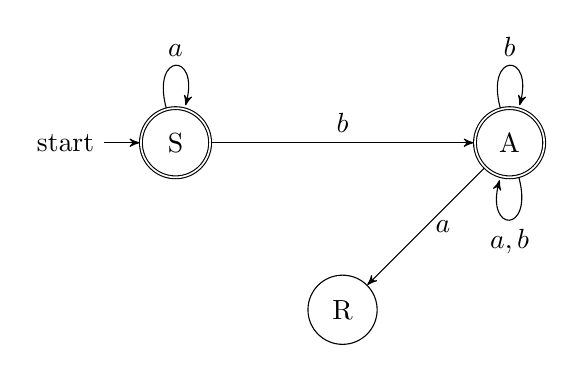
\begin{tikzpicture}[node distance=3cm]
    \node[initial, accepting, state] (1) {S};
    \node[state] (2) [below right of=1] {R};
    \node[state, accepting] (3) [above right of=2] {A};

    \draw (1) edge[loop above] node[align=center]{$a$} (1)
    	  (1) edge[above] node[align=center]{$b$} (3)
    	  (3) edge[loop above] node[align=center]{$b$} (3)
    	  (3) edge[right] node[align=center]{$a$} (2)
    	  (3) edge[loop below] node[align=center]{$a,b$} (3);
    \end{tikzpicture}
\end{center}

How would we do this if we instead of have the language
\[ L_2 = \{ a^n b^n : n \ge 0 \}? \]
It may be shown that such a language cannot be recognized by a deterministic finite automaton. To create an automaton that does recognize it, we require an additional \emph{stack}, which gives rise to the \emph{pushdown automaton}. The automaton itself is almost identical to the above automaton, except that we `push' an $a$ onto the stack when we read an $a$, and `pop' an $a$ when we read a $b$. Finally, we further require that the stack is empty when the string has been read.\\

We also have what is known as a \emph{context-free grammar}. We have a bunch of rules, and generate strings in the language by repetitively performing a replacement using one of the rules. It turns out that these are equivalent to pushdown automata.\\

Finally, consider the language
\[ L_3 = \{a^nb^nc^n : n \ge 0\}. \]
This cannot be recognized by even a pushdown automaton. This leads to the \emph{Turing machine}, where instead of a stack we have a `tape'. This represents the `ultimate' computer that can do anything a computer can do. We shall look at each of these in detail over the next few sections.\\

The focus of our study shall be each of the following.

\begin{center}
\begin{tabular}{|c|c|}
	\hline Machine & Language \\
	\hline
	Discrete finite automaton (DFA/FSA) & Regular expressions \\
	Pushdown automaton (PDA) & Context-free grammars \\
	Turing machine (TM) & Unrestricted grammars \\
	\hline
\end{tabular}
\end{center}

We can further introduce non-determinism in each of the three automata. We shall see that the expressive power of DFAs and TMs do not change on allowing non-determinism, while that of PDAs does.\\

First, before explaining anything, let us set up some notation and definitions for the rest of this course.

\begin{fdef}
	An \emph{alphabet} $\Sigma$ is a non-empty set. Its elements are referred to as \emph{letters} or \emph{terminals}.\\
	The set $\Sigma^*$ is the set of all finite strings over $\Sigma$. In particular, $\Sigma^*$ contains the empty string denoted $\epsilon$. The set $\Sigma^+$ is equal to $\Sigma^* \setminus \{\epsilon\}$.\\
	A \emph{language} is a subset of $\Sigma^*$.
\end{fdef}

The \emph{Chomsky hierarchy} represents the increasing complexity of languages. At the lowest level, we have \emph{regular languages} that are recognized by \emph{finite state automata}. This is a subset of \emph{context-free grammars}, which are recognized by \emph{pushdown automata}. This in turn is a subset of \emph{unrestricted grammars}, which are recognized by \emph{Turing machines}.\\

A finite state automaton is a tuple $(Q,\Sigma,\delta,q_0,F)$, where $Q$ is a finite non-empty set of states, $\Sigma$ is an alphabet, $\delta : Q \times \delta \to Q$ is the transition function, $q_0 \in Q$ is the initial state, and $F \subseteq Q$ is the set of accepting states.\\

Next, let us consider the language $\{a^nb^n : n \ge 0\}$ we mentioned earlier. This can be recognized by the context-free grammar
\begin{align*}
	S &\to \epsilon \\
	S &\to aSb
\end{align*}
What this means is that beginning with the string $S$, we keep performing replacements using one of the two rules above until our current string is composed of only terminals.\\
Another example is that of the set of non-empty strings with matched parentheses:
\begin{align*}
	S &\to () \\
	S &\to (S) \\
	S &\to SS
\end{align*}

A context-free grammar is a tuple $(V,\Sigma,R,S)$, where $V$ is a set of \emph{non-terminals} or \emph{variables}, $\Sigma$ is the alphabet, $R : V \to (V \cup \Sigma)^*$ is the finite set of \emph{rules}, and $S \in V$ is the \emph{start symbol}. The language of this grammar is the set of all strings (over terminals) derivable using the rules.\\

Finally, let us look at unrestricted grammars. Consider the language $\{a^nb^nc^n : n \ge 1\}$. This can be represented by the unrestricted grammar
\begin{align*}
	S &\to abc \\
	S &\to aAbc \\
	Ab &\to bA \\
	Ac &\to Bbcc \\
	bB &\to Bb \\
	aB &\to aa \\
	aB &\to aaA
\end{align*}
The only difference between unrestricted and context-free grammars is that the former allow the left-hand side of the rules to be strings as well. That is, an unrestricted grammar is a tuple $(V,\Sigma,R,S)$, where $V$ is a set of non-terminals, $\Sigma$ is the alphabet, $R : (V \cup \Sigma)^* \to (V \cup \Sigma)^*$ is the finite set of rules, and $S \in V$ is the start symbol. As before, the language of this grammar is the set of all strings (over terminals) derivable using the rules.\\

\section{Integration}

\subsection{Basic definitions}

	\subsubsection{Integrals of real functions}

		First, let us recall the definition of the Riemann\footnote{technically the Darboux integral?} integral of functions on $\R$.

		\begin{fdef}[Riemann Integral]
			Let $[a,b]$ be a given interval. A \emph{partition} $\mathcal{P}$ of $[a,b]$ is a finite set of points $x_0,x_1,\ldots,x_n$ where
			\[ a = x_0 \le x_1 \le \cdots \le x_{n-1} \le x_n = b.  \]
			We also write $\Delta x_i = x_i - x_{i-1}$ for $i = 1,2,\ldots,n$.\\
			For a bounded real function $f$ on $[a,b]$ and each partition $\mathcal{P}$ of $[a,b]$, we set
			\[ M_i = \sup_{x_{i-1} \le x \le x_i} f(x), \qquad m_i = \inf_{x_{i-1} \le x \le x_i} f(x). \]
			Further, set
			\[ U(\mathcal{P},f) = \sum_{i=1}^{n} M_i \Delta x_i, \qquad L(\mathcal{P},f) = \sum_{i=1}^n m_i \Delta x_i \]
			as the upper and lower Riemann sum respectively,
			and finally,
			\[ \overline{\int_a^b} f \dif x = \inf_{\mathcal{P}} U(\mathcal{P},f), \qquad \underline{\int_a^b} f \dif x = \sup_{\mathcal{P}} L(\mathcal{P},f) \]
			as the upper and lower Riemann integrals of $f$.\\
			cc
		\end{fdef}

		Next, we define the slightly more general Riemann-Stieltjes integral. Note that this is the same as the usual Riemann integral when $\alpha$ is the identity function.

		\begin{fdef}[Riemann-Stieltjes Integral]
			Let $\alpha : [a,b] \to \R$ be a monotonically increasing function on $[a,b]$. Corresponding to each partition $\mathcal{P}$ of $[a,b]$, write $\Delta \alpha_i = \alpha(x_i) - \alpha(x_{i-1})$. Clearly, $\Delta \alpha_i \ge 0$ for each $i$.\\
			For any real function $f$ which is bounded on $[a,b]$, we put
			\[ U(\mathcal{P},f,\alpha) = \sum_{i=1}^n M_i \Delta \alpha_i, \qquad L(\mathcal{P},f,\alpha) = \sum_{i=1}^n m_i \Delta \alpha_i, \]
			where $M_i,m_i$ are defined as in the definition of the Riemann integral. We then define
			\[ \overline{\int_a^b} f \dif \alpha = \inf_{\mathcal{P}} U(\mathcal{P},f,\alpha), \qquad \underline{\int_a^b} f \dif \alpha = \sup_{\mathcal{P}} L(\mathcal{P},f,\alpha). \]
			If these two are equal, we say that $f$ is \emph{Riemann-Stieltjes integrable} with respect to $\alpha$ on $[a,b]$ and denote the common value as $\int_a^b f \dif \alpha$.
		\end{fdef}

		We also remark that
		\[ \int_a^b f \dif \alpha = \lim_{\max \Delta \alpha_k \to 0} \sum_{k=1}^n f(\tau_k) \Delta \alpha_k, \]
		where $x_{k-1} \le \tau_k \le x_k$ for each $k$.\\
		More generally, we define the \emph{mesh} of $\mathcal{P}$ with respect to $\alpha$ as
		\[ \norm{\mathcal{P}} = \max\{ \Delta\alpha_i : 1 \le i \le n \}. \]
		So for all $\epsilon > 0$, there exists $\delta > 0$ such that for any partition $\mathcal{P}$ of $[a,b]$ with $\norm{P} < \delta$, then
		\[ \left| \sum_{k=1}^n f(\tau_k) \Delta\alpha_k - \int_a^b f \dif \alpha \right| < \epsilon \]
		for any choice of points $x_{k-1} \le \tau_k \le x_k$.

	\subsubsection{Riemann-Stieltjes integrals of complex-valued functions}

		\begin{fdef}
			A function $\gamma : [a,b] \to \C$ for $[a,b] \subseteq \R$ is said to be of \emph{bounded variation} if there exists $M > 0$ such that for any partition $\mathcal{P} = \{ a = t_0 < t_1 < \cdots < t_{m-1} < t_m = b \}$ of $[a,b]$,
			\[ v(\gamma;\mathcal{P}) = \sum_{k=1}^m |\gamma(t_k) - \gamma(t_{k-1})| \le M. \]
			The \emph{total variation} $V(\gamma)$ of $\gamma$ is defined by
			\[ V(\gamma) = \sup \{ v(\gamma;\mathcal{P}) : \mathcal{P}\text{ is a partition of }[a,b] \}. \]
			Clearly, $V(\gamma) \le M < \infty$.
		\end{fdef}

		\begin{lemma}
			Let $\gamma : [a,b] \to \C$ be of bounded variation. Then,
			\begin{enumerate}
				\item If $\mathcal{P},\mathcal{Q}$ are partitions of $[a,b]$ with $\mathcal{P} \subseteq \mathcal{Q}$, then $v(\gamma;\mathcal{P}) \le v(\gamma;\mathcal{Q})$.
				\item If $\sigma : [a,b] \to \C$ is also of bounded variation and $\alpha,\beta\in\C$, then $\alpha\gamma + \beta\sigma$ is of bounded variation and
				\[ V(\alpha\gamma + \beta\sigma) \le |\alpha| V(\gamma) + |\beta| V(\sigma). \]
			\end{enumerate}
		\end{lemma}
		We omit the proof of the above, which is direct on using the triangle inequality on the definition of $v(\gamma;\mathcal{P})$.

		\begin{lemma}
			If $\gamma : [a,b] \to \C$ is piecewise smooth, $\gamma$ is of bounded variation and
			\[ V(\gamma) = \int_a^b |\gamma'(t)| \dif t. \]
		\end{lemma}
		\begin{proof}
			It suffices to show the required in the case where $\gamma$ is smooth, since in general we can consider the refinement of any partition that splits along the pieces along which $\gamma$ is smooth.\\
			The right hand side is well-defined since $\gamma'$ is continuous. Let $\mathcal{P} = \{ a = t_0 < t_1 < \cdots < t_{m-1} < t_m = b \}$. By definition,
			\begin{align*}
				v(\gamma,\mathcal{P}) &= \sum_{k=1}^m |\gamma(t_k) - \gamma(t_{k-1})| \\
					&= \sum_{k=1}^m \left| \int_{t_{k-1}}^{t_k} \gamma'(t) \dif t \right| \\
					&\le \sum_{k=1}^m \int_{t_{k-1}}^{t_k} |\gamma'(t)| \dif t = \int_a^b |\gamma'(t)| \dif t.
			\end{align*}
			Therefore, $V(\gamma) \le \int_a^b |\gamma'(t)| \dif t$, so $\gamma$ is of bounded variation.\\
			Since $\gamma'$ is continuous, it is uniformly continuous. So, if $\epsilon > 0$, we may choose $\delta_1 > 0$ such that
			\[ |s-t| < \delta_1 \implies |\gamma'(s) - \gamma'(t)| < \epsilon. \]
			Also, let $\delta_2 > )$ such that if $\norm{P} < \delta_2$, then
			\[ \left| \int_a^b |\gamma'(t)| \dif t - \sum_{k=1}^m |\gamma'(\tau_k)| (t_k - t_{k-1}) \right| < \epsilon, \]
			where $\tau_k$ is any point in $[t_{k-1},t_k]$. Therefore,
			\begin{align*}
				\int_a^b |\gamma'(t)| \dif t &\le \epsilon + \sum_{k=1}^{m} |\gamma'(t_k)| (t_k - t_{k-1}) \\
					&= \epsilon + \sum_{k=1}^m \left| \int_{t_{k-1}}^{t_k} \gamma'(\tau_k) \dif t \right| \\
					&\le \epsilon + \sum_{k=1}^m \left| \int_{t_{k-1}}^{t_k} (\gamma'(\tau_k) - \gamma'(t)) \dif t \right| + \sum_{k=1}^m \left| \int_{t_{k-1}}^{t_k} \gamma'(t) \dif t \right|.
			\end{align*}
			If $\norm{P} < \delta = \min(\delta_1,\delta_2)$, then $|\gamma'(\tau_k) - \gamma'(t)| < \epsilon$ for all $t \in [t_{k-1},t_k]$ and
			\begin{align*}
				\int_a^b |\gamma'(t) \dif t| &\le \epsilon + \epsilon(b-a) + \sum_{k=1}^{m} |\gamma(t_k) - \gamma(t_{k-1})| \\
					&= \epsilon(1 + b-a) + V(\gamma;P) \le \epsilon(1 + b-a) + V(\gamma),
			\end{align*}
			so we are done since $1+b-a > 0$ is finite and $\epsilon$ can be made arbitrarily small.
		\end{proof}

		\begin{ftheo}
			Let $\gamma : [a,b] \to \C$ be of bounded variation and suppose that $f : [a,b] \to \C$ is continuous. Then, there exists a (unique) complex number $\mathcal{I}$ such that for every $\epsilon > 0$, there exists $\delta > 0$ such that when $\mathcal{P} = \{ t_0 < t_1 < \cdots < t_m \}$ is a partition of $[a,b]$ with $\norm{P} = \max_{1 \le k \le m} (t_k - t_{k-1}) < \delta$,
			\[ \left| \mathcal{I} - \sum_{k=1}^m f(\tau_k) (\gamma(t_k) - \gamma(t_{k-1})) \right| < \epsilon \]
			for any choice of points $\tau_k$ with $t_{k-1} \le \tau_k \le t_k$.\\
			This $\mathcal{I}$ is called the integral of $f$ with respect to $\gamma$ over $[a,b]$ and is denoted by
			\[ \mathcal{I} = \int_a^b f \dif \gamma = \int_a^b f(t) \dif\gamma(t). \]
		\end{ftheo}
		\begin{proof}
			First of all, note that it suffices to consider the case where $\gamma$ is real-valued, since we can write $\gamma = \gamma_1 + \iota \gamma_2$, where $\gamma_1,\gamma_2$ are real-valued, to get two integrals $\mathcal{I}_1,\mathcal{I}_2$ (for $\gamma_1,\gamma_2$ respectively), and finally use the triangle inequality to get $\mathcal{I} = \mathcal{I}_1 + \iota\mathcal{I}_2$.\\
			Since $f$ is continuous, it is uniformly continuous. We can (inductively) find positive numbers $\delta_1 > \delta_2 > \cdots $ such that if $|s-t| < \delta_m$, $|f(s) - f(t)| < 1/m$. For each $M \ge 1$, let $\mathcal{P}_m$ be the collection of all partitions of $[a,b]$ with $\norm{P} \le \delta_m$, so $\mathcal{P}_1 \supseteq \mathcal{P}_2 \supseteq \cdots \supseteq \mathcal{P}_m \supseteq \cdots$. Finally, define $F_m$ to be the closure of the set
			\[ \{ \sum_{k=1}^n f(\tau_k) (\gamma(t_k) - \gamma(t_{k-1})) : P \in \mathcal{P}_m \text{ and } t_{k-1} \le \tau_k \le t_k \}. \]
			First note, that because $\mathcal{P}_1 \supseteq \mathcal{P}_2 \supseteq \cdots$, it follows trivially that
			\[ F_1 \supseteq F_2 \supseteq \cdots. \]
			We claim that
			\begin{align}
				\diam F_m &\le \frac{2}{m} V(\gamma). \label{eqn: diam-bound}
			\end{align}
			If we do this, then Cantor's Theorem (since $\C$ is complete) implies that there is precisely one complex number $\mathcal{I}$ such that $\mathcal{I} \in F_m$ for all $m \ge 1$. Then, for any $\epsilon > 0$, we may let $m > (2/\epsilon)V(\gamma)$ so $\epsilon > (2/m) V(\gamma) \ge \diam F_m$. Since $\mathcal{I} \in F_m$, $F_m \subseteq B(\mathcal{I},\epsilon)$. Therefore, $\delta = \delta_m$ gets the job done.\\
			To show \Cref{eqn: diam-bound}, it suffices to show that
			\[ \diam \left\{ f(\tau_k) \left( \gamma(t_k) - \gamma(t_{k-1}) \right) : P \in \mathcal{P}_m \text{ and } \right\} \le \frac{2}{m} V(\gamma). \]
			To do this, if $P = \{ t_0 < \cdots < t_n \}$ is a partition, denote by $S(P)$ a sum of the form $\sum f(\tau_k) \left( \gamma(t_k)  - \gamma(t_{k-1})\right)$ where $t_{k-1} \le \tau_k \le t_k$ for each $k$. Fixing $m \ge 1$, let $P \in \mathcal{P}_m$. If $P \subseteq Q$ (so $Q \in \mathcal{P}_m$ as well), then
			\[ |S(P) - S(Q)| < \frac{1}{m} V(\gamma). \]
			We only show this in the case where $Q$ is obtained from $P$ by adding a single extra partition point (the general case follows similarly). Let $Q = \{ t_0 < t_1 < \cdots < t_{p-1} < t^* < t_p < \cdots t_n \}$. If $t_{p-1} \le \sigma \le t^*$ and $t^* \le \sigma' \le t_p$. Then,
			\[ S(Q) = \sum_{k \ne p} f(\sigma_k) ( \gamma(t_k) - \gamma(t_{k-1}) ) + f(\sigma) \left( \gamma(t^*) - \gamma(t_{p-1}) \right) + f(\sigma') \left( \gamma(t_p) - \gamma(t^*) \right). \]
			Then, using the definition of $\delta_m$,
			\begin{align*}
				\left| S(P) - S(Q) \right| &= \left| \sum_{k\ne p} \left( f(\tau_k) - f(\sigma_k) \right) \left( \gamma(t_k) - \gamma(t_{k-1}) \right) \right. \\
				&\qquad\left. + f(\tau_p) (\gamma(t_p) - \gamma(t_{p-1})) - f(\sigma)(\gamma(t^*) - \gamma(t_{p-1})) - f(\sigma')( \gamma(t_p) - \gamma(t^*) ) \right| \\
				&\le \frac{1}{m} \sum_{k \ne p} |\gamma(t_k) - \gamma(t_{k-1}| + \left| \left( f(\tau_p) - f(\sigma) \right) \left( \gamma(t^*) - \gamma(t_{p-1}) \right) + \left( f(\tau_p) - f(\sigma') \right) \left( \gamma(t_p) - \gamma(t^*) \right) \right| \\
				&\le \frac{1}{m} \sum_{k \ne p} \left| \gamma(t_k) - \gamma(t_{k-1}) \right| + \frac{1}{m} \left| \gamma(t^*) - \gamma(t_{p-1}) \right| + \frac{1}{m} \left| \gamma(t_p) - \gamma(t^*) \right| \\
				&\le \frac{1}{m} V(\gamma).
			\end{align*}

			Next, let $P,R$ be any two partitions in $R$, and $Q - P \cup R$ a partition that contains $P$ and $R$. Using the first part,
			\[ |S(P) - S(Q)| \le |S(P) - S(Q)| + |S(Q) - S(R)| \le \frac{2}{m} V(\gamma). \]
			It follows that the diameter of the set of interest is at most $(2/m) V(\gamma)$, completing the proof.
		\end{proof}

		\begin{ftheo}
			Let $f,g$ be continuous functions on $[a,b]$ and let $\gamma,\sigma$ be functions of bounded variation on $[a,b]$. Then for any scalars $\alpha,\beta$,
			\begin{align*}
				\int_a^b (\alpha f + \beta g) \dif \gamma &= \alpha \int_a^b f \dif \gamma + \beta \int_a^b g \dif \gamma \\
				\int_a^b f \dif( \alpha\gamma + \beta\sigma ) = \alpha\int_a^b f \dif \gamma + \beta\int_a^b f \dif \sigma.
			\end{align*}
		\end{ftheo}

		% \begin{proof}
		% 	It follows near-directly that $\int_a^b \alpha f \dif \gamma = \alpha \int_a^b f \dif \gamma$ (just use $|\alpha|\epsilon$ instead of $\epsilon$ in the definition). So, to show \Cref{eqn: scalar-addition-closure of fn int}, it suffices to show it for $\alpha = \beta = 1$. To do this, use $\epsilon/2$ in the definitions of integrability, and take $\delta = \min\{\delta_1,\delta_2\}$ (where $\delta_1,\delta_2$ are the values obtained from the integrability of $f,g$).\\
		% 	Similarly, $\int_a^b f \dif (\alpha \gamma) = \alpha \int_a^b f \dif \gamma$ and $\int_a^b f \dif(\gamma+\sigma) = \int_a^b f \dif \gamma + \int_a^b f \dif \sigma$.
		% \end{proof}

		\begin{lemma}
			\label{lemma: can split integral}
			Let $\gamma : [a,b] \to \C$ be of bounded variation and let $f : [a,b] \to \C$ be continuous. If $a = t_0 < t_1 < \cdots < t_{n-1} < t_n = b$, then
			\[ \int_a^b f \dif \gamma = \sum_{k=1}^n \int_{t_{k-1}}^{t_k} f \dif \gamma. \]
		\end{lemma}

		We omit the proofs of the above.

		\begin{ftheo}
			If $\gamma$ is piecewise smooth and $f : [a,b] \to \C$ is continuous, then $\int_a^b f \dif \gamma = \int_a^b f(t) \gamma'(t) \dif t$.
		\end{ftheo}
		\begin{proof}
			It suffices to consider the case where $\gamma$ is smooth by \Cref{lemma: can split integral}. Also, by looking at the real and imaginary parts of $\gamma$ separately, it suffices to consider the case where $\gamma$ is real-valued on $[a,b]$. Let $\epsilon > 0$ and choose $\delta > 0$ such that $P = \{ a = t_0 < t_1 < \cdots < t_n = b \}$ has $\norm{P} < \delta$, then
			\[ \left| \int_a^b f \dif \gamma - \sum_{k=1}^n f(\tau_k) (\gamma(t_k) - \gamma(t_{k-1})) \right| < \epsilon/2 \]
			for any $t_{k-1} \le \tau_k \le t_k$ for each $k$.\\
			Applying the mean value theorem on $\gamma$ (this requires that $\gamma$ be real-valued), one gets that there exists $\tau_k \in [t_{k-1},t_k]$ for each $k$ such that
			\[ \gamma'(\tau_k) = \frac{\gamma(t_k) - \gamma(t_{k-1})}{t_k - t_{k-1}}. \]
			Using these $\tau_k$ specifically, 
			\[ \left| \int_a^b f \dif \gamma - \sum_{k=1}^n f(\tau_k) \gamma'(\tau_k) (t_k - t_{k-1}) \right| < \epsilon/2 \]
		\end{proof}

\subsection{Integrals On Curves}

	\begin{fdef}
		$\gamma:[a,b]\to\C$ is called a \emph{rectifiable path} if it is continuous and of bounded variation. Note that if $\gamma$ is piecewise smooth, then it is rectifiable and its length is
		\[ \int_a^b |\gamma'(t)| \dif t = V(\gamma). \]
	\end{fdef}

	\begin{fdef}
		If $\gamma : [a,b] \to \C$ is a rectifiable path and $f$ is a function continuous on $[a,b]$, then the \emph{(line) integral} of $f$ along $\gamma$ is
		\[ \int_a^b f(\gamma(t)) \dif \gamma(t). \]
		This line integral is also denoted as
		\[ \int_\gamma f = \int_\gamma f(z) \dif z \]
	\end{fdef}

	For example, if $\gamma:[0,2\pi] \to \C$ as $\gamma(t) = e^{\iota t}$,
	\[ \int_\gamma \frac{1}{z} \dif z = \int_0^{2\pi} e^{-\iota t} (\iota e^{\iota t}) \dif t = 2 \pi \iota. \]
	and
	\[ \int_\gamma z^m \dif z = \int_0^{2\pi} e^{\iota m t} (\iota e^{\iota t}) \dif t = \iota \int_0^{2\pi} \cos((m+1)t) \dif t - \int_0^{2\pi} \sin((m+1)t) \dif t = 0. \]

	\begin{theorem}
		If $\gamma : [a,b] \to \C$ is a rectifiable path and $\varphi : [c,d] \to [a,b]$ is a continuous non-decreasing function with $\varphi(c) = a, \varphi(d) = b$, then for any function $f$ continuous on $\gamma$,
		\[ \int_\gamma f = \int_{\gamma \circ \varphi} f. \]
	\end{theorem}

	\begin{remark}
		The above uses the fact that $\gamma \circ \varphi$ is also rectifiable (Why is this true?).
	\end{remark}

	\begin{proof}
		Let $\epsilon > 0$ and choose $\delta_1 > 0$ such that for a partition $\{ s_0 < s_1 < \cdots  < s_n \}$ of $[c,d]$ with $(s_{k} - s_{k-1}) < \delta_1$ and any $s_{k-1} \le \sigma_k \le s_k$,
		\[ \left| \int_{\gamma \circ \varphi} f - \sum_{k=1}^{n} f((\gamma \circ \varphi)(s_k)) - f((\gamma \circ \varphi)(s_{k-1})) \right| < \epsilon/2. \]
		Similarly, choose $\delta_2 > 0$ such that for a partition $\{ t_0 < t_1 < \cdots < t_m \}$ of $[a,b]$ with $(t_k - t_{k-1}) < \delta_2$ and $t_{k-1} \le \tau_k \le t_k$,
		\[ \left| \int_{\gamma} f - \sum_{k=1}^{m} f(\gamma(t_k)) - f(\gamma(t_{k-1})) \right| < \epsilon/2. \]
		Since $\varphi$ is uniformly continuous on $[c,d]$, there exists $\delta > 0$ less than $\delta_1$ such that $|\varphi(s) - \varphi(t)| < \delta_2$ whenever $|s-t| < \delta$. So, if $\{ s_0 < s_1 < \cdots < s_n \}$ is a partition of $[c,d]$ with $(s_k - s_{k-1}) < \delta < \delta_1$ and $t_k = \varphi(s_k)$, then $\{ t_0 < t_1 < \cdots < t_n \}$ is a partition of $[a,b]$ with $(t_k - t_{k-1}) < \delta_2$. If $s_{k-1} \le \sigma_k \le s_k$ and $\tau_k = \varphi(\sigma_k)$, then we can use the two earlier inequalities to conclude that
		\[ \left| \int_\gamma f - \int_{\gamma \circ \varphi} f \right| < \epsilon, \]
		completing the proof.
	\end{proof}

	\begin{definition}
		Let $\gamma : [a,b] \to \C$ be a rectifiable path, and for $a \le t \le b$, set $|\gamma|(t) = V(\gamma;[a,t])$. That is,
		\[ |\gamma|(t) = \sup\left\{ \sum_{k=1}^{n} |\gamma(t_k) - \gamma(t_{k-1})| : \{ t_0 < t_1 < \cdots < t_n \}\text{ is a partition of }[a,t] \right\}. \]
		Clearly, $|\gamma|$ is increasing on $[a,b]$ and of bounded variation. In fact, $V(|\gamma|;[a,b]) = |\gamma|(b) - |\gamma|(a)$. If $f$ is continuous on $[a,b]$, define
		\[ \int f |\dif z| = \int_a^b f(\gamma(t)) \dif |\gamma|(t). \]
	\end{definition}

	\begin{ftheo}
		Let $\gamma$ be a rectifiable curve and suppose that $f$ is a function continuous on $\{\gamma\}$. Then,
		\begin{equation}
			\label{eqn: 2.2}
			\int_\gamma f = - \int_{-\gamma} f,
		\end{equation}
		\begin{equation}
			\label{eqn: 2.3}
			\left| \int_\gamma f \right| \le \int_\gamma |f| |\dif z| \le V(\gamma) \sup\{ |f(z)| : z \in \{\gamma\} \},
		\end{equation}
		and for $c \in \C$,
		\begin{equation}
			\label{eqn: 2.4}
			\int_\gamma f(z) \dif z = \int_{\gamma + c} f(z-c) \dif z.
		\end{equation}
	\end{ftheo}
	\begin{proof}
		\Cref{eqn: 2.2,eqn: 2.4} follow near-directly from the definition, so we prove only \Cref{eqn: 2.3}. Let $\epsilon > 0$. Then, there exists $\delta > 0$ such that if $P = \{ t_0 < t_1 < \cdots t_n \}$ is a partition of $[a,b]$ with $\norm{P} < \delta$, then
		\begin{align*}
			\left| \left| \int_\gamma f(z) \dif z \right| - \left| \sum_{k=1}^n f(\gamma(\tau_k)) (\gamma(t_k) - \gamma(t_{k-1})) \right| \right| &\le \left| \int_\gamma f(z) \dif z - \sum_{k=1}^n f(\gamma(\tau_k)) (\gamma(t_k) - \gamma(t_{k-1})) \right| \\
			&< \epsilon/2
		\end{align*}
		for any $t_{k-1} \le \tau_k \le t_k$.
		That is,
		\begin{align*}
			\left| \int_\gamma f(z) \dif z \right| &< \left| \sum_{k=1}^n f(\gamma(\tau_k)) (\gamma(t_k) - \gamma(t_{k-1})) \right| + \epsilon/2 \\
			&\le  \sum_{k=1}^n \left| f(\gamma(\tau_k)) \right| \left|\gamma(t_k) - \gamma(t_{k-1}) \right| + \epsilon/2.
		\end{align*}
		We may also assume that for this same $\delta$,
		\[  . \]
		Recall that $|\gamma|(t)$ is an increasing function. So,
		\[ |\gamma(t_k)| - |\gamma|(t_{k-1}) \ge |\gamma(t_k) - \gamma(t_{k-1})| \]
		Therefore,
		\begin{align*}
			\left| \int_\gamma f(z) \dif z \right| &< \sum_{k=1}^n |f(\gamma(\tau_k))| \left( |\gamma|(t_k) - |\gamma|(t_{k-1}) \right) + \epsilon/2 \\
				&< \int_\gamma |f(z)| |\dif z| + \epsilon.
		\end{align*}
		It follows that
		\[ \left| \int_\gamma f(z) \dif z \right| \le \int_\gamma |f(z)| |\dif z|. \]
		To conclude the proof, note that
		\[ \int_\gamma |\dif z| = |\gamma|(b) - |\gamma|(a) = |\gamma|(b) = V(\gamma), \]
		so
		\[ \int_\gamma |f(z)| |\dif z| \le V(\gamma) \sup_{z \in \{\gamma\}} |f(z)|. \]
	\end{proof}

	\begin{flem}
		\label{lemma: polygonal}
		If $G$ is an open set in $\C$, $\gamma : [a,b] \to G$ is a rectifiable path, and $f : G \to \C$ is continuous, then for every $\epsilon > 0$ there exists a polygonal path $\Gamma$ in $G$ such that $\Gamma(a) = \gamma(a)$, $\Gamma(b) = \gamma(b)$, and
		\[ \left| \int_\gamma f - \int_\Gamma f \right| < \epsilon \]
	\end{flem}
	\begin{proof}
		We prove the result in the case where $G$ is an open disk. In the general case where $G$ need not be a disk, since $\{\gamma\}$ is compact, there exists a number $r$ with $0 < r < d(\{\gamma\},\partial G)$. Choose $\delta > 0$ such that $|\gamma(s) - \gamma(t)| < r$ when $|s-t| < \delta$. The idea is that we shall take several smaller disks and stitch together the polygonal paths on each of these sections.\\
		If $P = \{ t_0 < t_1 < \cdots < t_n \}$ is a partition of $[a,b]$ with $\norm{P} < \delta$, then $|\gamma(t_k) - \gamma(t_{k-1})| < r$ for $t_{k-1} \le t \le t_k$. That is, if $\gamma_k : [t_{k-1}, t_k] \to G$ is defined by $\gamma_k(t) = \gamma(t)$, then $\{\gamma_k\} \subseteq B(\gamma(t_{k-1}),r)$ for $1 \le k \le n$. Getting a polygonal path $\Gamma_k$ for each $k$ such that
		\[ \left| \int_{\gamma_k} f - \int_{\Gamma_k} f \right| < \epsilon/n, \]
		defining $\Gamma(t) = \Gamma_k(t)$ on $[t_{k-1},t_k]$ does the job.
		\\

		Now, let us prove the result in the disk case.\\
		Because $\{\gamma\}$ is a compact set, $d = d(\{\gamma\},\partial G) > 0$. It follows that if $G = B(c,r)$, then $\{\gamma\} \subseteq B(c,\rho)$ where $\rho = r - d/2$.\\
		Now, observe that $f$ is uniformly continuous on $\overline{B}(c,\rho) \subseteq G$. Thus, we may assume without loss of generality that $f$ is uniformly continuous on $G$. Now, choose $\delta > 0$ such that if $|z-w| < \delta$, then $|f(z) - f(w)| < \epsilon$. If $\gamma : [a,b] \to G$, then $\gamma$ is uniformly continuous so there is a partition $P = \{t_0 < t_1 < \cdots < t_n\}$ of $[a,b]$ such that if $t_{k-1} \le s,t \le t_k$, $|\gamma(s) - \gamma(t)| < \delta$, and such that for $t_{k-1} \le \tau_k \le t_k$,
		\[ \left| \int_\gamma f - \sum_{k=1}^n f(\gamma(\tau_k)) (\gamma(t_k) - \gamma(t_{k-1})) \right| < \epsilon. \]
		Now, define $\Gamma : [a,b] \to G$ by
		\[ \Gamma(t) = \frac{(t_k - t) \gamma(t_{k-1}) + (t - t_{k-1}) \gamma(t_k)}{t_k - t_{k-1}} \]
		if $t_{k-1} \le t \le t_k$. This is the polygonal path we shall consider. Indeed,
		\begin{align*}
			\Gamma(t) - \gamma(\tau_k) &= \frac{t_k - t}{t_k - t_{k-1}} (\gamma(t_{k-1}) - \gamma(\tau_k)) + \frac{t - t_{k-1}}{t_k - t_{k-1}} (\gamma(t_k) - \gamma(\tau_k)),
		\end{align*}
		so
		\begin{align*}
			|\Gamma(t) - \gamma(\tau_k)| &\le \left| \frac{t_k - t}{t_k - t_{k-1}} \right| \left| \gamma(t_{k-1}) - \gamma(\tau_k) \right| + \left| \frac{t - t_{k-1}}{t_k - t_{k-1}} \right| \left| \gamma(t_k) - \gamma(\tau_k) \right| \\
				&\le \left| \gamma(t_{k-1}) - \gamma(\tau_k) \right| + \left| \gamma(t_k) - \gamma(\tau_k) \right| < 2\delta.
		\end{align*}
		Thus,
		\begin{align*}
			\int_\Gamma f &= \int_a^b f(\Gamma(t)) \Gamma'(t) \dif t \\
				&= \sum_{k-1}^n \frac{\gamma(t_k) - \gamma(t_{k-1})}{t_k - t_{k-1}} \int_{t_{k-1}}^{t_k} f(\Gamma(t)) \dif t
		\end{align*}
		and
		\begin{align*}
			\left| \int_\gamma f - \int_\Gamma f \right| &= \left| \int_\gamma f - \sum_{k=1}^n f(\gamma(\tau_k)) (\gamma(t_k) - \gamma(t_{k-1})) \right| + \left| \sum_{k=1}^n f(\gamma(\tau_k)) (\gamma(t_k) - \gamma(t_{k-1})) - \int_\Gamma f \right| \\
				&\le \epsilon + \left| \sum_{k=1}^n f(\gamma(\tau_k)) (\gamma(t_k) - \gamma(t_{k-1})) - \int_\Gamma f \right| \\
				&\le \epsilon + \sum_{k=1}^n \frac{|\gamma(t_k) - \gamma(t_{k-1})|}{t_k - t_{k-1}} \int_{t_{k-1}}^{t_k} |f(\Gamma(t)) - f(\gamma(\tau_k))| \dif t \\
				&\le \epsilon + \epsilon \sum_{k=1}^n |\gamma(t_k) - \gamma(t_{k-1})| \\
				&\le \epsilon (1 + V(\gamma)),
		\end{align*}
		which can be made arbitrarily small, thus completing the proof.
	\end{proof}

	The following can be thought of as an analogue of the Fundamental Theorem of Calculus for complex functions.

	\begin{ftheo}
		Let $G$ be open in $\C$ and $\gamma$ be a rectifiable path in $G$ with initial and end points $\alpha,\beta$. If $f : G \to \C$ is a continuous function with a primitive $F : G \to \C$ ($F$ is differentiable and $F' = f$), then
		\[ \int_\gamma F = F(\beta) - F(\alpha). \]
	\end{ftheo}
	\begin{proof}
		When $\gamma : [a,b] \to \C$ is piecewise smooth,
		\begin{align*}
			\int_\gamma f &= \int_a^b f(\gamma(t)) \gamma'(t) \dif t \\
				&= \int_a^b F'(\gamma(t)) \gamma'(t) \dif t \\
				&= \int_a^b (F \circ \gamma)'(t) \dif t \\
				&= (F \circ \gamma) (b) - (F \circ \gamma) (a) & \text{(by the Fundamental Theorem of Calculus)} \\
				&= F(b) - F(a).
		\end{align*}
		In general, we may use \Cref{lemma: polygonal}. For $\epsilon > 0$, let $\Gamma$ be a polygonal path of the described form. Since $\Gamma$ is piecewise smooth, $\int_\Gamma f = F(\beta) - F(\alpha)$, so
		\[ \left| \int_\gamma f - (F(\beta) - F(\alpha)) \right| < \epsilon. \]
		Since $\gamma$ was chosen arbitrarily, the desideratum follows.
	\end{proof}

	The fundamental theorem of calculus says that each continuous function has a primitive. However, this is not true for functions of complex variables. For example, letting $f(z) = |z|^2$, if $F$ is a primitive of $f$, then $F$ is analytic. So, if $F = U + \iota V$, $x^2 + y^2 = F'(x+\iota y)$. Consequently,
	\begin{align*}
		\dpd{U}{x} &= \dpd{V}{y} = x^2 + y^2 \\
		\dpd{U}{y} &= \dpd{V}{x} = 0.
	\end{align*}
	However, $\pd{U}{y} = 0$ implies that $U(x,y) = u(x)$ for some function $u$, which implies that $u'(x) = x^2 + y^2$, a contradiction.

\subsection{Power series representation of analytic functions}

	Recall the following result which we had used in the proof of \Cref{theo: open disk harmonic conjugate}.

	\begin{theorem}
		Let $\varphi : [a,b] \times [c,d] \to \C$ be a continuous function and defined $g : [c,d] \to \C$ by
		\[ g(t) = \int_a^b \varphi(s,t) \dif s. \]
		Then $g$ is continuous. Moreover, if $\pd{\varphi}{t}$ exists and is a continuous function on $[a,b] \times [c,d]$, then $g$ is continuously differentiable and
		\[ g'(t) = \int_a^b \dpd{\varphi}{t}(s,t) \dif s. \]
	\end{theorem}

	This is referred to as the Leibniz rule.\\

	For example, this may be used to prove that if $|z| < 1$,
	\[ \int_0^{2\pi} \frac{e^{\iota s}}{e^{\iota s} - z} = 2 \pi. \]
	To do so, let $\varphi(s,t) = e^{\iota s} / (e^{\iota s} - tz)$ for $0 \le t \le 1$ and $0 \le s \le 2\pi$. Observe that $\varphi$ is continuously differentiable since $|z| < 1$. Thus,
	\[ g(t) = \int_0^{2\pi} \varphi(s,t) \dif s \]
	is continuously differentiable. Since $\varphi(s,0) = 1$, $g(0) = 2\pi$. Now,
	\begin{align*}
		g'(t) &= \int_0^{2\pi} \dpd{\varphi}{t}(s,t) \dif s \\
			&= \int_0^{2\pi} \frac{ze^{\iota s}}{(e^{\iota s} - tz)^2}.
	\end{align*}
	For fixed $t$, $\Phi(s) = z\iota/(e^{\iota s} - tz)$ satisfies
	\[ \Phi'(s) = -\frac{\iota z}{(e^{\iota s} - tz)^{2}} \cdots \iota e^{\iota s} = \frac{ze^{\iota s}}{(e^{\iota s} - tz)^2}. \]
	Therefore, $g'(t) = \Phi(2\pi) - \Phi(0) = 0$, so $g$ is a constant and $g(t) = g(0) = 2\pi$ for any $t$, $1$ in particular.

	\begin{prop}
		Let $f : G \to \C$ be analytic and suppose that $\overline{B(a,r)} \subseteq G$ for some $r > 0$. If $\gamma(t) = a + re^{\iota t}$ for $ 0 \le t \le 2\pi$, then
		\[ f(z) = \frac{1}{2\pi\iota} \int_\gamma \frac{f(w)}{w - z} \dif w \]
		for $|z-a| < r$.
	\end{prop}
	\begin{proof}
		Defining $G_1 = \left\{ (z-a)/r : z \in G \right\}$ and $g(z) = f(a + r z)$, it suffices to consider the case where $a = 0$ and $r = 1$.\\
		Fix $z$ with $|z| < 1$. It must be shown that
		\[ f(z) = \int_{2\pi\iota} \int_\gamma \frac{f(w)}{w-z} \dif w = \frac{1}{2\pi} \int_0^{2\pi} \frac{f(e^{\iota s} e^{\iota s})}{e^{\iota s} - z} \dif s. \]
		That is, we want to show that
		\begin{align*}
			 0 &= \int_0^{2\pi} \frac{f(e^{\iota s}) e^{\iota s}}{e^{\iota s} - z} \dif s - 2 \pi f(z) \\
			 	&= \int_0^{2\pi} \left(\frac{f(e^{\iota s}) e^{\iota s}}{e^{\iota s} - z} - f(z)\right) \dif s.
		\end{align*}
		For this, let
		\[ \varphi(s,t) = \frac{f(z + t(e^{\iota s} - z)) e^{\iota s}}{e^{\iota s} - z} - f(z) \]
		for $0 \le t \le 1$ and $0 \le s \le 2\pi$, and
		\[ g(t) = \int_0^{2\pi} \varphi(s,t) \dif s. \]
		We wish to show that $g(1) = 0$. Observe that
		\[ g(0) = \int_0^{2\pi} \frac{f(z) e^{\iota s}}{e^{\iota s} - z} - f(z) \dif s = f(z) \int_0^{2\pi} \frac{e^{\iota s}}{e^{\iota s} - z} \dif s - 2\pi f(z) = 0. \]
		Also,
		\begin{align*}
			g'(t) &= \int_0^{2\pi} \dpd{\varphi}{t}(s,t) \dif s \\
				&= \int_0^{2\pi} \frac{e^{\iota s}}{e^{\iota s} - z} f'(z + t(e^{\iota s} - z)) (e^{\iota s} - z) \dif s \\
				&= \int_0^{2\pi} e^{\iota s} f'(z + t(e^{\iota s - z})) \dif s \\
				&= \frac{1}{t} f(z + t(e^{\iota s} - z)) \Biggr|_{s=0}^{s=2\pi} \\
				&= 0,
		\end{align*}
		completing the proof.
	\end{proof}

	If $|z-a| = r$ and $w$ is on the circle $|w-a| = r$, then
	\[ \frac{1}{w-z} = \frac{1}{w-a} \cdot \frac{1}{1 - \frac{z-a}{w-a}} = \frac{1}{w-a} \sum_{i=0}^{\infty} \left( \frac{z-a}{w-a} \right)^i. \]

\end{document}